\input{style/sqt.tex}

\title{How to Count}
\subtitle{Combinatorics Revisited}
\institute{Sydney Quant Traders}
\date{}

\begin{document}

\maketitle

\section{Fundamentals}

\begin{frame}{Counting Problem Examples}
  \begin{itemize}
    \item How many outfits can be made from 4 shirts and 3 hats?
    \item How many ways to arrange 4 people on a circular table?
    \item How many ways to choose a set of 3 cards out of a deck?
    \item How many ways to divide 10 students into 3 teams of non-zero size?
    \item How many bracelets can be made with 3 white and 3 black beads?
    \item How many colorings of a graph with the colors \{red, green, blue\} 
    such that no edge connects two vertices of the same color.
  \end{itemize}
\end{frame}

\begin{frame}{Introductory Problem}
  \textcolor{sqt-question}{
    \textbf{Example:} How many outfits can be made from 4 shirts and 3 hats?}\\
  Count the number of ways to construct/configure an outfit.\\
  Each step of the construction/configuration process requires a \textbf{decision}.\\
  \begin{center}
    \includegraphics[width=13cm]{assets/outfits.pdf}
  \end{center}
\end{frame}

\begin{frame}{Configuration}
  \begin{sqt:definition}[\textbf{Definition:} configuration]
    A configuration is a way (i.e. sequence of decisions) to construct an object.
  \end{sqt:definition}

  Each leaf node in a decision tree corresponds to a different configuration.

  \begin{center}
    \includegraphics[width=10cm]{assets/outfits.pdf}
  \end{center}
\end{frame}

\begin{frame}{Equivalence Relation}
  \textcolor{sqt-question}{
    \textbf{Example:} How many ways to arrange 3 people on a circular table?\\
    Two arrangements are identical if one can be obtained
    from the other by rotation.
  }

  \begin{center}
    \includegraphics[width=9cm]{assets/circular_seating.pdf}
  \end{center}
\end{frame}

\begin{frame}{Equivalence Relations}
  Let $X$ be the set of configurations.
  A counting quesiton may specify what it means for two configurations $x_1, x_2\in X$ to be considered equal.\\
  In other words, it provides an equivalence relation on the set $X$ of configurations.

  \begin{sqt:definition}[\textbf{Definition:} equivalence relation]
    A relation $\sim$ is an equivalence relation if it satisfies
    \begin{itemize}
      \item reflexive
      \item symmetric
      \item transitive
    \end{itemize}
  \end{sqt:definition}


\end{frame}

\begin{frame}{Equivalence Class}
  \begin{sqt:definition}[\textbf{Definition:} equivalence class]
    The equivalence class of $x$ under $\sim$ is denoted by $[x]_\sim$.\\
    It is defined as the set of all elements equivalent to $x$ under $\sim$.
  \end{sqt:definition}
\end{frame}

\begin{frame}{Quotient Set}
  \begin{sqt:definition}[\textbf{Definition:} quotient set]
    The quotient set of $X$ under $\sim$ is denoted by $idk$.\\
    It is defined as the set of all equivalence classes (under $\sim$) of its elements.
  \end{sqt:definition}
\end{frame}

\begin{frame}{Counting Problems}
  \begin{sqt:definition}[Definition: counting problem]
    Determining the size of the quotient set of a specified set $X$ of configurations,
    modulo some specified equivalence relation $\sim$.
  \end{sqt:definition}
\end{frame}

\section{Perms and Combs}

\begin{frame}{Techniques}
  \begin{itemize}
    \item stars and bars
    \item principle of inclusion exclusion
    \item double counting
    \item bijections
    \item number of possible words
  \end{itemize}
\end{frame}

\section{Group Actions}

\section{Generating Functions}

\end{document}